\documentclass[12pt]{beamer}
\usepackage[utf8]{inputenc} % style d'écriture
\usepackage[T1]{fontenc}      % package
\usepackage[french]{babel}  % package pour langue française
\usepackage{graphicx}
\usepackage{subcaption}
\usepackage{url}
\usepackage{color}
\usepackage{geometry}
\usepackage{amssymb}
\usepackage{multirow, makecell}
\usepackage{listings}

% William PENSEC, étudiant en Master 2 LSE 2020/2021

\usetheme[secheader]{Madrid}
\beamertemplatenavigationsymbolsempty
\setbeamertemplate{frametitle continuation}{}

\lstset{
  aboveskip=5mm,
  belowskip=-2mm,
  basicstyle=\footnotesize,
  breakatwhitespace=false,
  breaklines=true,
  captionpos=b,
  commentstyle=\color{red},
  deletekeywords={...},
  escapeinside={\%*}{*)},
  extendedchars=true,
  framexleftmargin=16pt,
  framextopmargin=3pt,
  framexbottommargin=6pt,
  frame=tb,
  keepspaces=true,
  keywordstyle=\color{blue},
  language=C++,
  literate=
  {²}{{\textsuperscript{2}}}1
  {⁴}{{\textsuperscript{4}}}1
  {⁶}{{\textsuperscript{6}}}1
  {⁸}{{\textsuperscript{8}}}1
  {€}{{\euro{}}}1
  {é}{{\'e}}1
  {è}{{\`{e}}}1
  {ê}{{\^{e}}}1
  {ë}{{\"{e}}}1
  {É}{{\'{E}}}1
  {Ê}{{\^{E}}}1
  {û}{{\^{u}}}1
  {ù}{{\`{u}}}1
  {â}{{\^{a}}}1
  {à}{{\`{a}}}1
  {á}{{\'{a}}}1
  {ã}{{\~{a}}}1
  {Á}{{\'{A}}}1
  {Â}{{\^{A}}}1
  {Ã}{{\~{A}}}1
  {ç}{{\c{c}}}1
  {Ç}{{\c{C}}}1
  {õ}{{\~{o}}}1
  {ó}{{\'{o}}}1
  {ô}{{\^{o}}}1
  {Õ}{{\~{O}}}1
  {Ó}{{\'{O}}}1
  {Ô}{{\^{O}}}1
  {î}{{\^{i}}}1
  {Î}{{\^{I}}}1
  {í}{{\'{i}}}1
  {Í}{{\~{Í}}}1,
  morekeywords={*,...},
  numbers=left,
  numbersep=10pt,
  numberstyle=\tiny\color{black},
  rulecolor=\color{black},
  showspaces=false,
  showstringspaces=false,
  showtabs=false,
  stepnumber=1,
  stringstyle=\color{gray},
  tabsize=4,
  title=\lstname,
}

\title[Compte rendu de stage n\textsuperscript{o}12]{Coopération de drones dans un système hétérogène}
\subtitle{Compte rendu de stage n\textsuperscript{o}12}
\author{William \textsc{Pensec}}
%\author{William \textsc{Pensec}}
%\author{William \textsc{Pensec}}
\institute[Lab-STICC]{Lab-Sticc}
\date{\today}

\AtBeginSection[]
{
\begin{frame}<beamer>{Sommaire}
\tableofcontents[currentsection,currentsubsection, 
    hideothersubsections, 
    sectionstyle=show/shaded,
]
\end{frame}
}

\begin{document}
	% ---------------------------------------------------------------- %
	\begin{frame}
		\begin{titlepage}
			\begin{figure}[H]
				\centering
				
\includegraphics[scale=.15]{labsticc.png}
				\hspace{3cm}
				
\includegraphics[scale=.3]{ubo.png}
			\end{figure}
		\end{titlepage}
	\end{frame}
	
	% ---------------------------------------------------------------- %
	\section*{Sommaire}
	\begin{frame}
		\frametitle{Sommaire}
		\begin{center}
			\tableofcontents
		\end{center}
	\end{frame}
	%
	% ---------------------------------------------------------------- %
	\section{Schémas}
	\begin{frame}
    	    % Point de départ (x,y,z), point d'arrivée (x1,y1,z1)
    	    % Déplacement en bypassant le GPS et système de naviguation du drone
    	    % Calcul de l'angle entre les 2 points et envoi des commandes de déplacement pour aller en diagonale
    	    % Déplacement vers l'axe z puis x puis y (par exemple)
    	    \begin{figure}
			    \centering
			    \includegraphics[width=0.8\textwidth]{piecePosTraj.png}
			\end{figure}
	\end{frame}
	%
	% ---------------------------------------------------------------- %
	\section{Exploration de l'utilisation de la boussole}
	\begin{frame}
	    \begin{block}{}
	        \begin{itemize}
	            \setbeamertemplate{itemize item}[triangle]
	            \item Fonction  : getCompassData() => Supported Platforms : M210V2, M300 mais code non protégé dans le SDK
	            \item Boussole initialisée en même temps que l'IMU avant le décollage
	                \begin{itemize}
	                    \setbeamertemplate{itemize item}[cercle]
	                    \item Manuellement : mouvement spécifique demandée par l'application
	                    \item Par programmation : aucune information de comment faire dans la documentation
	                \end{itemize}
	           \item Vitesse limitée en intérieure (très faible)
	        \end{itemize}
	    \end{block}
	\end{frame}
	%
	% ---------------------------------------------------------------- %
	\section{Exemples de la caméra du Raspberry Pi}
	\begin{frame}[allowframebreaks]
        \begin{figure}
            \centering
            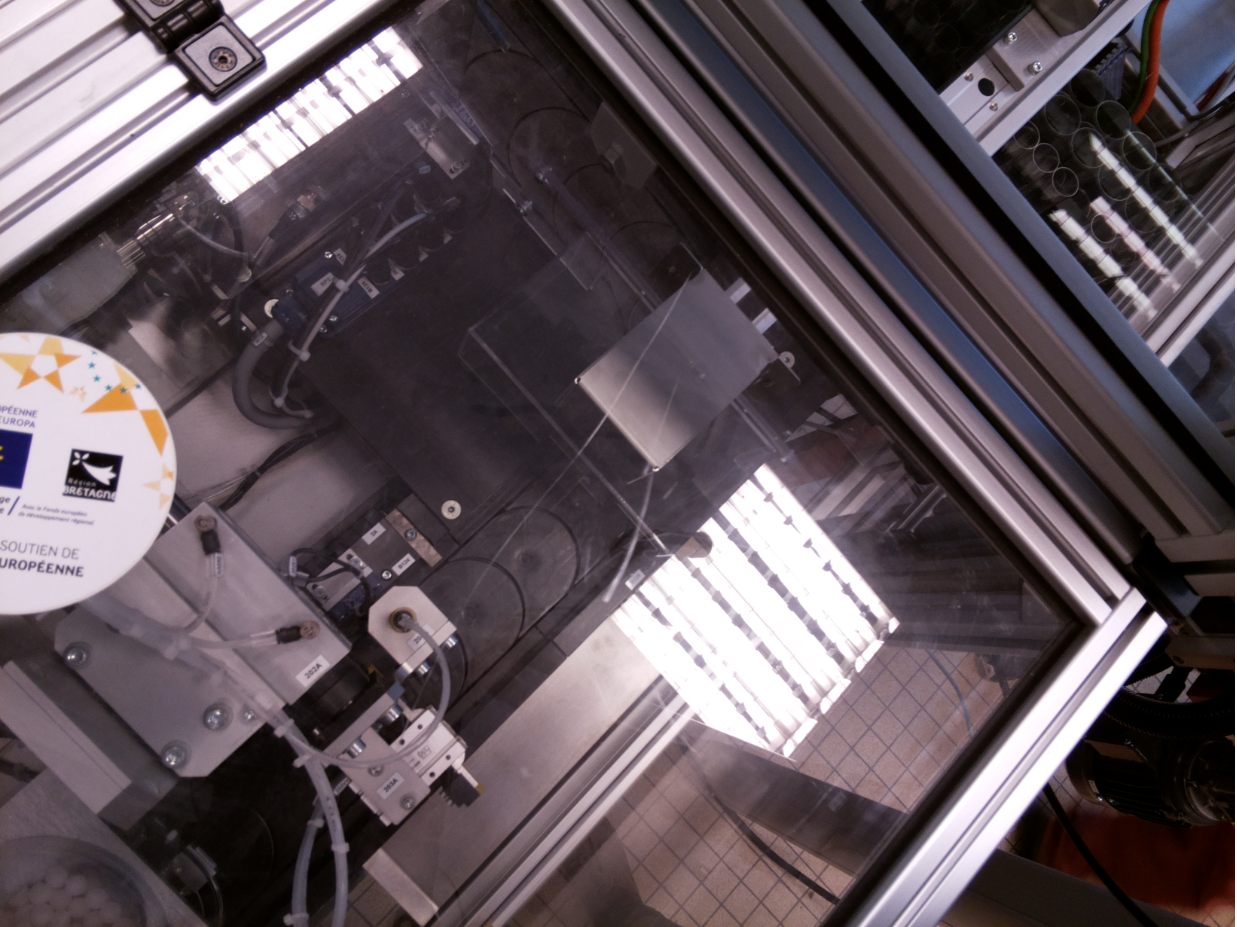
\includegraphics[width=0.7\textwidth]{imageStatioInf1.png}
            \caption*{Photo prise au-dessus de la plate-forme en simulant un vol stationnaire}
        \end{figure}
        
        \begin{figure}
            \centering
            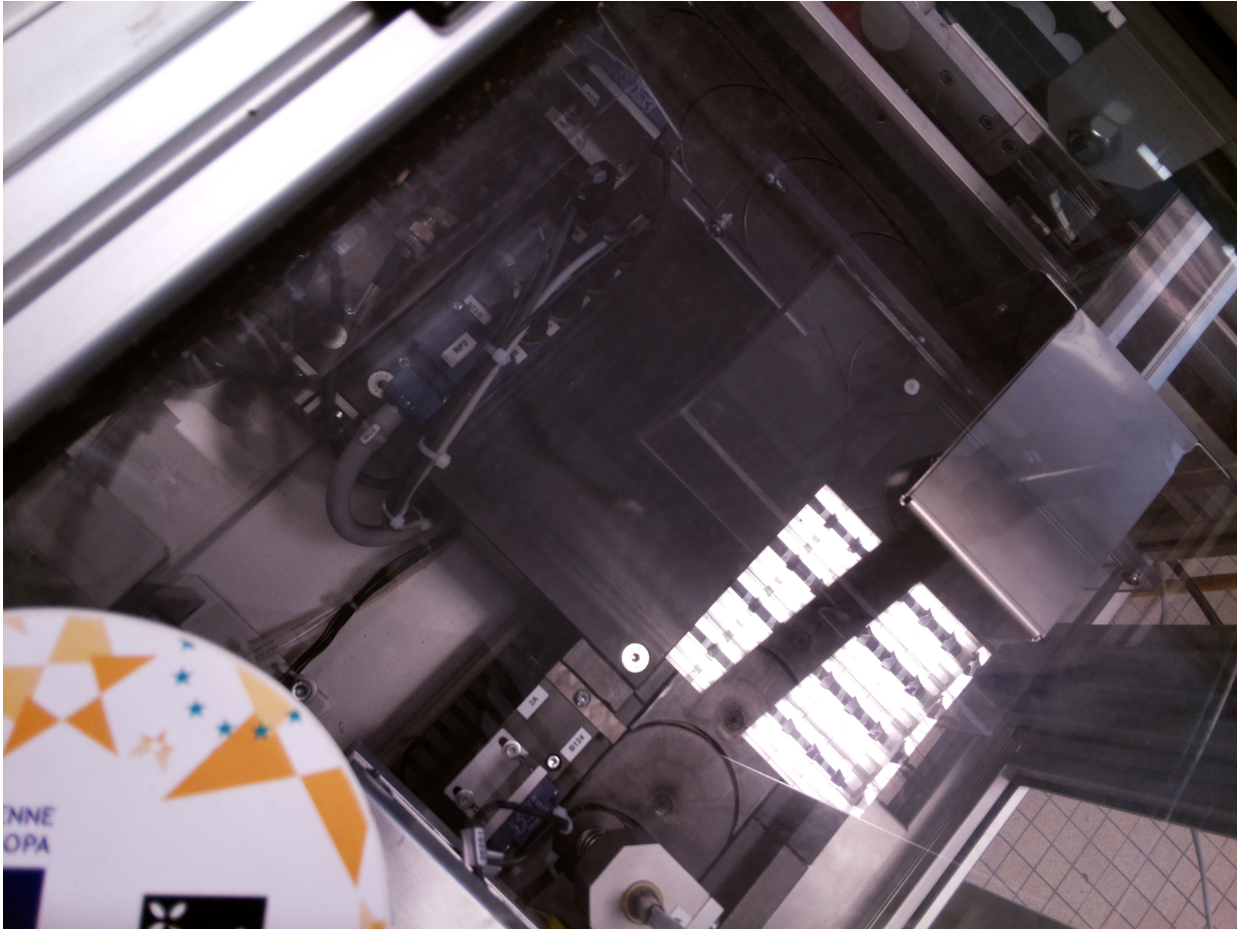
\includegraphics[width=0.7\textwidth]{imageStatioInf2.png}
            \caption*{Photo prise sur la plate-forme}
        \end{figure}
        
        \begin{figure}
            \centering
            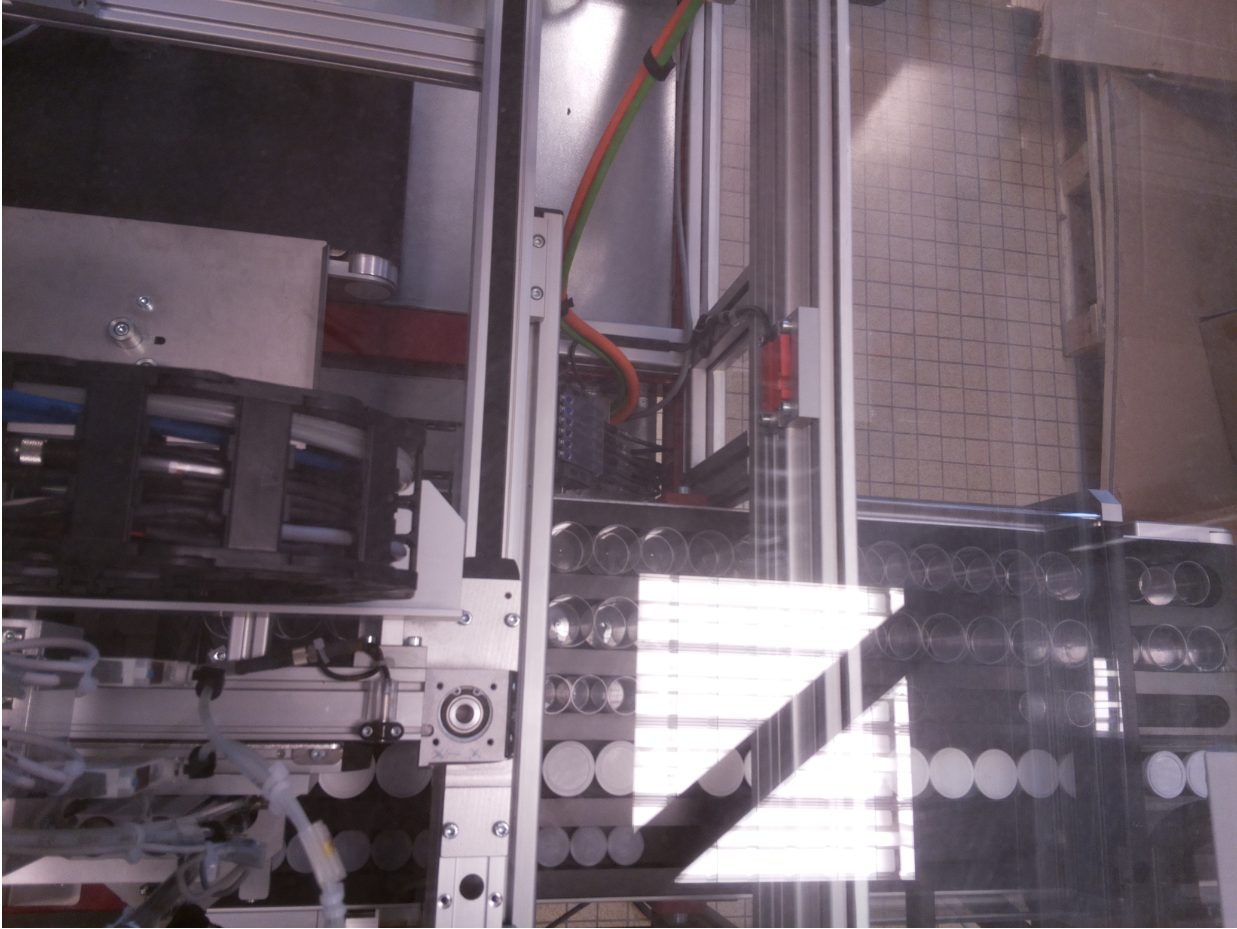
\includegraphics[width=0.7\textwidth]{imageStationnaireSup1.png}
            \caption*{Photo prise sur la plate-forme}
        \end{figure}
        
        \begin{figure}
            \centering
            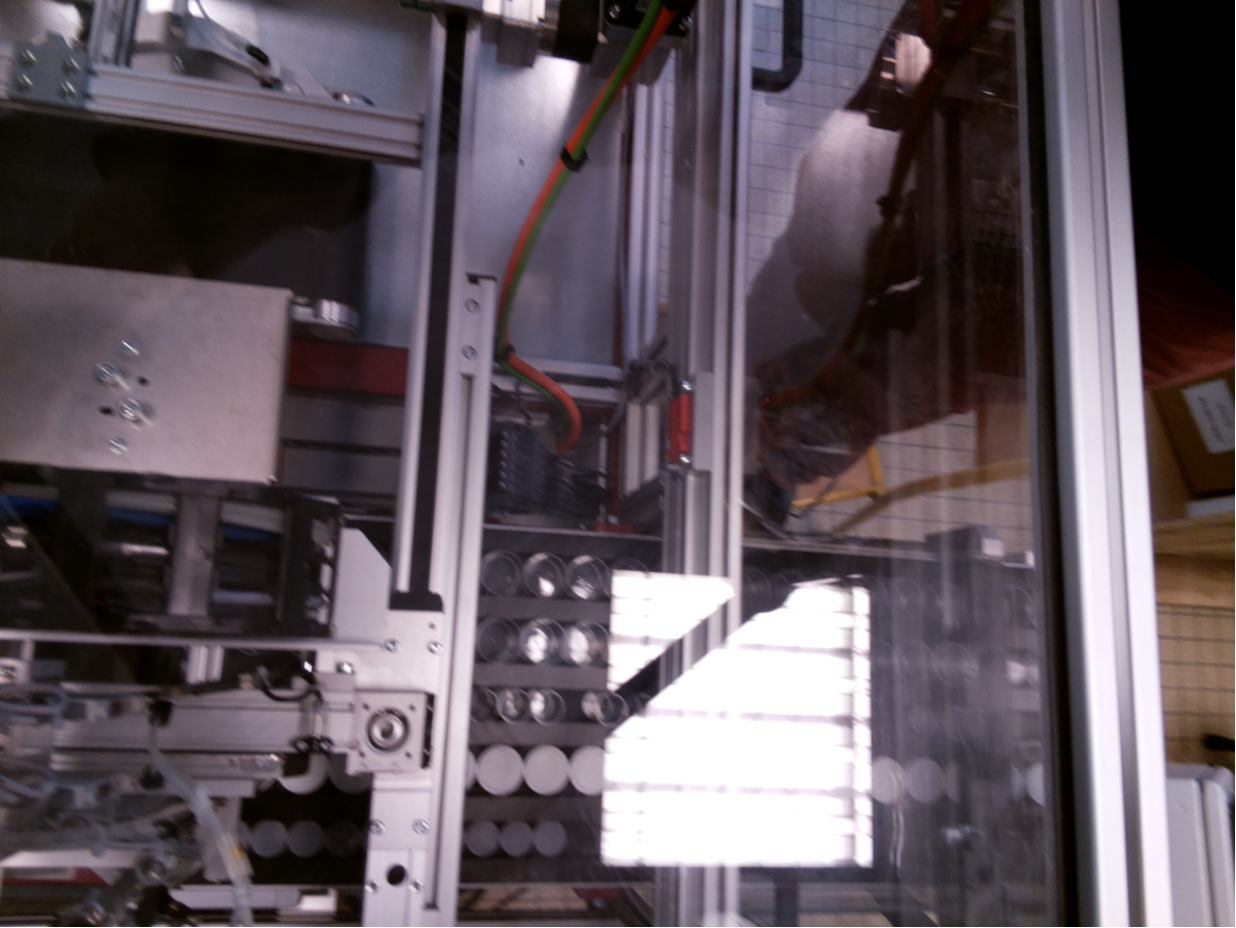
\includegraphics[width=0.7\textwidth]{imageStatioSup1.png}
            \caption*{Photo prise au-dessus de la plate-forme en simulant un vol (mouvements du drone dans les 3 axes}
        \end{figure}
        
        \begin{figure}
            \centering
            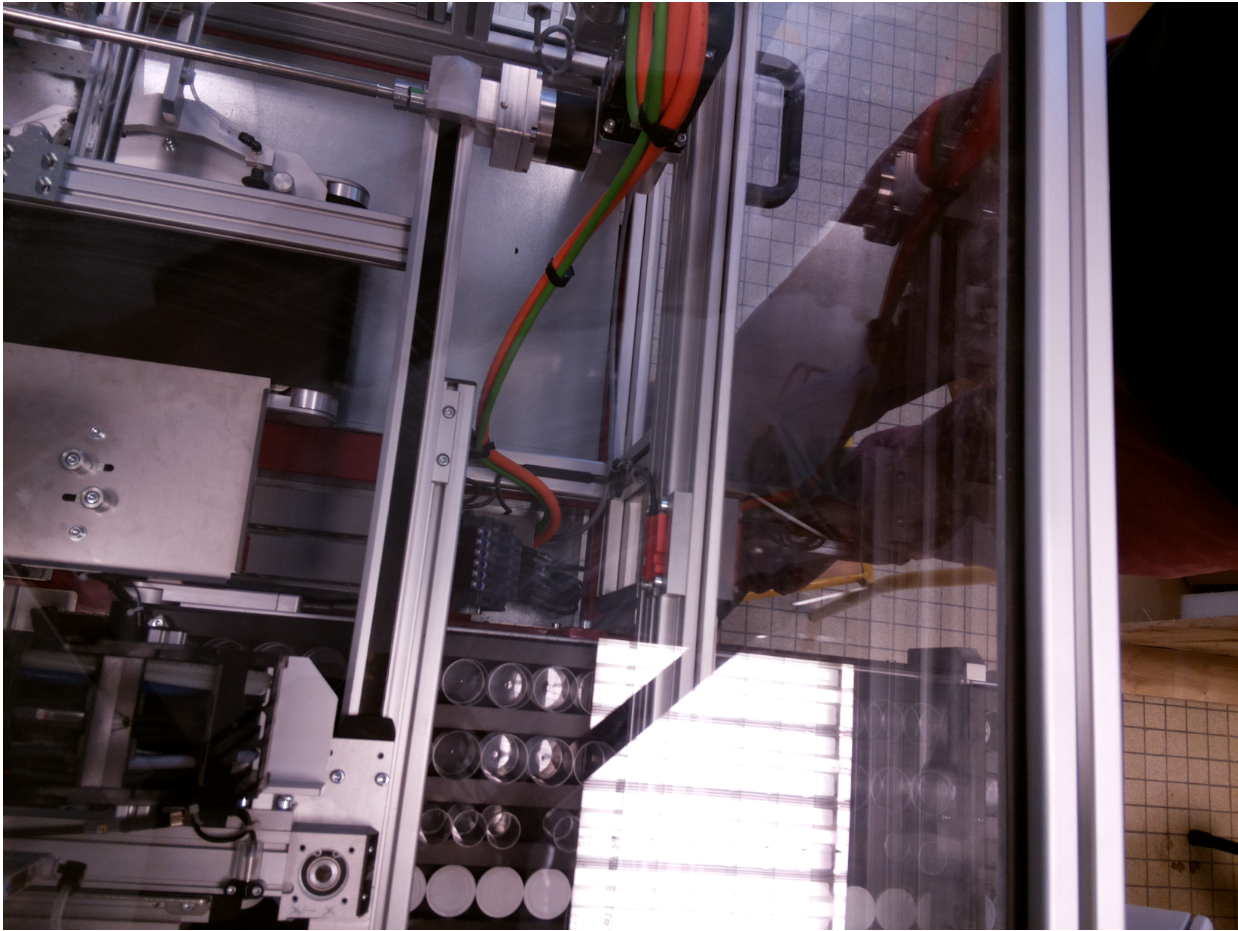
\includegraphics[width=0.7\textwidth]{imageStatioSup2.png}
            \caption*{Photo prise au-dessus de la plate-forme en simulant un vol}
        \end{figure}
        
        \begin{figure}
            \centering
            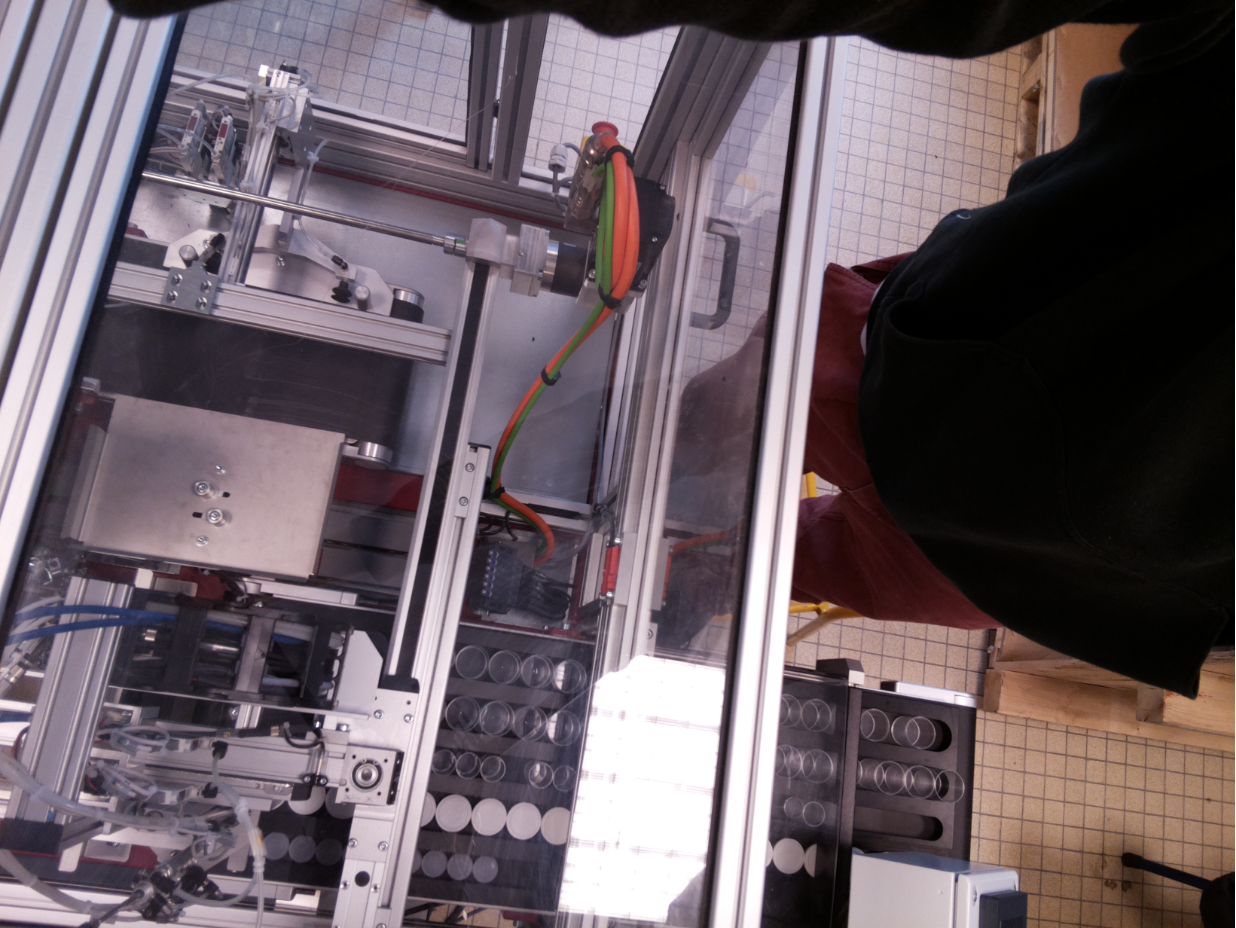
\includegraphics[width=0.7\textwidth]{imageStatioSup3.png}
            \caption*{Photo prise au-dessus de la plate-forme en simulant un vol}
        \end{figure}	
	\end{frame}
	%
	%% ---------------------------------------------------------------- %
\end{document}